\chapter{Введение}

\textbf{Актуальность.} Изменения в городской среде требуют формирования новых механизмов 
планирования инфраструктуры города. Для получения эффективных результатов, следует осуществлять 
принятие решений на основе актуальных данных, отражающих предпочтения жителей. В рамках 
магистерской диссертации следует разработать метод построения маршрутов общественного транспорта 
на основе предпочтений жителей.

\textbf{Цель работы} -- разработка метода генерации маршрутов общественного транспорта на основе 
предпочтений жителей для минимизации дискомфорта перемещения в городе.

\textbf{Теоретический этап} -- рассмотрение информации по существующим алгоритмам, свободных систем 
маршрутизации; составление теоретической базы проекта и систематизация полученных знаний; 
составление технического задания. 

\textbf{Практический этап} -- реализация системы на основе теоретической базы, составленной ранее с 
использование технического задания.

\textbf{Финальный этап} -- внедрение готового продукта, получение обратной информации и исправление 
ошибок.

\textbf{Теоретические задачи:}
\vspace*{-1em}
\begin{itemize}\itemsep-5pt
    \item разработка алгоритма формирования маршрутов на основе имеющихся данных;
    \item выбор критериев качества для оценки построенных маршрутов;
    \item методы построение маршрута по заданным критериям;
    \begin{itemize}\itemsep-5pt
        \item предпочтения жителей;
        \item длина маршрута;
        \item дискомфорт перемещения;
        \item и др.
    \end{itemize}
    \item разработка критериев для оценки качества построенного маршрута;
\end{itemize}
\textbf{Практические задачи:}
\vspace*{-1em}
\begin{itemize}\itemsep-5pt
    \item разработка механизма генерация исходных данных;
    \item реализация разработанных алгоритмов и методов;
    \item отображение результатов генерации маршрутов на карте;
    \item оценка качества построенных маршрутов.
\end{itemize}

\newpage

\textbf{Понятийный аппарат}
\vspace*{-1em}
\begin{itemize}\itemsep-5pt
    \item \textbf{framework (фреймворк)} -- программная платформа, определяющая структуру 
        программной системы; программное обеспечение, облегчающее разработку и объединение разных 
        компонентов большого программного проекта.
    \item \textbf{OpenStreetMap (OSM)} -- некоммерческий веб-картографический проект по созданию 
        силами сообщества участников-пользователей Интернета подробной свободной и бесплатной 
        географической карты мира.
    \item \textbf{OSRM} -- фреймворк для вычисления кратчайших путей в графе дорог. Разработана 
        для использования с картографическим сервисом OSM.
    \item \textbf{node (точка)} -- точка с указанными координатами;
    \item \textbf{way (линия)} -- упорядоченный список точек, составляющих линию или полигон;
    \item \textbf{relation (отношение)} -- группы точек, линий и других отношений, которым 
        назначаются некоторые свойства;
    \item \textbf{tag (тег)} -- пары <<ключ -- значение>>, могут назначаться точкам, линиям и 
        отношениям.
\end{itemize}

\textbf{Объект исследования} -- построения маршрутов общественного транспорта на основе актуальных 
данных о предпочтениях жителей по перемещениям в современной городской среде.

\textbf{Предмет исследования} -- методы построения маршрутов общественного транспорта учитывающие 
актуальные данные о предпочтениях жителей по перемещению и интенсивности пассажиропотоков в городе.

\chapter{Описание решаемых задач}
В данной работе рассматриваются к решению следующие задачи:
\begin{enumerate}\itemsep-5pt
    \item генерация псевдореалистичных данных кластеров предпочтений;
    \item разработка метода маршрутизации между кластерами предпочтений;
    \item модификация и использование существующих алгоритмов для задачи маршрутизации;
    \item разработка критериев оценки качества построенных маршрутов;
    \item представление построенных маршрутов на карте;
\end{enumerate}

Первая задача заключается в создании псевдореалистичных данных для замены отсутствующий реальных 
на данный момент. Они нужны для работы над последующими задачами как некий приближенный аналог.

Вторая задача заключается в разработке метода обхода кластеров предпочтений, который используя 
информацию о пассажиропотоках генерирует оптимальный список обхода кластеров. Метод будет 
основывается на эволюционных алгоритмах. На текущем этапе используется алгоритм имитации отжига 
для генерации субоптимальных списков обхода. В дальнейшем планируется задействовать алгоритм 
табу поиска и возможно разработка нового метода на их основе.

Третья задача заключается в анализе и модификации существующий алгоритмов поиска маршрутов из 
точки \( A \) в точку \( B \), но для применения на графе дорог с учётом рельефа и других 
специфичных городских препятствий. Используемый алгоритм должен быть оптимален по времени работы 
и требуемой памяти для частого построения маршрутов.

Четвёртая задача заключается в разработке критериев по которым можно будет оценить качество 
построенного маршрута. Также предоставить данную информацию пользователю и модуля построения 
маршрутов для последующей оптимизации.

Пятая задача заключается в разработке web-инструмента для отображения и редактирования построенных 
маршрутов по предыдущим пунктам.


Псевдокод текущий алгоритмов представлен в Приложении (\ref{ref:greedy}, 
\ref{ref:annealing}, \ref{ref:tabu})).

\chapter{Результат анализа и систематизации информации}
Среди различных источников информации мной были выделены следующая литература:

Route Planning in Transport Networks 
\url{http://research.microsoft.com/pubs/207102/MSR-TR-2014-4.pdf}\\
Статья хорошо описывающая алгоритмы, которые используются для построения маршрутов на графе дорог. 
В ней предоставлена информация по эффективности, производительности и алгоритмической сложности.
Даёт в основном обзорное представление по рассматриваемым алгоритмам, но даёт ссылки на литературу, 
в которой они рассмотрены более подробно.

Contraction Hierarchies: Faster and Simpler Hierarchical Routing in Road Networks 
\url{http://algo2.iti.kit.edu/schultes/hwy/contract.pdf}\\
Статья описывающая один из быстрых и наиболее простых алгоритмов маршрутизации на графе дорог: 
Contraction Hierarchies. В ней предоставлена исчерпывающая информация по его работе и методах на 
которых он основан. Также предоставлены результаты сравнения данного алгоритма с многими другими.

Генетические алгоритмы \url{http://mathmod.aspu.ru/images/File/ebooks/GAfinal.pdf}\\
В книге рассмотрены генетические алгоритмы, широко применяемые в последнее время для решения задач 
оптимизации. Описываются стандартные функции универсального пакета MATLAB 7.0.1, предназначенные 
для решения задач оптимизации с помощью генетических алгоритмов.

Генетический алгоритм для определения минимального времени пути в интеллектуальных транспортных 
система \url{http://masters.donntu.org/2010/fknt/kazakovaj/library/translate1.htm}\\
В данной статье описано использование генетического алгоритм для определения 
минимального времени движения с различными сценариями реальных условий дорожного движения и 
различной скоростью движения транспортного средства. Эффективность генетического алгоритма 
наглядно демонстрируется в применении на реальной карте современного города с очень большим 
числом вершин.

Алгоритмы решения задачи быстрого поиска пути на географических картах 
\url{http://engjournal.ru/articles/1054/1054.pdf}\\
В данной статье рассмотрены алгоритмы, позволяющие для подготовленного ландшафта предоставить 
один из возможных вариантов пути из одной точки в другую на географической карте с учетом 
особенностей проходимости местности. Описаны методы: алгоритмы поиска кратчайшего пути 
(Дейкстры); алгоритмы поиска субоптимального пути (A* и его модификации, в частности Theta*); 
алгоритмы постобработки маршрутов (удаление точек, лежащих на одной прямой; Line of Sight). 
Особое внимание уделено эвристическим алгоритмам, позволяющим найти близкий к оптимальному и в 
достаточной степени реалистично выглядящий маршрут. Описаны способы интерпретации ландшафта. 
Представлены выводы о применимости отдельных алгоритмов и их комбинаций.

\newpage

\chapter{Структура магистерской работы}
\begin{enumerate}\itemsep-5pt
    \item Введение
    \vspace*{-1em}
    \begin{itemize}\itemsep-5pt
        \item Актуальность
        \item Цели, задачи
        \item Ожидаемый результат
    \end{itemize}
    \item Введение в проблему синтеза маршрутов
    \vspace*{-1em}
    \begin{itemize}\itemsep-5pt\itemsep-5pt
        \item Анализ предметной области
        \item Состояние современных исследований
        \item Требования к методам
    \end{itemize}
    \item Метод построения маршрутов
    \vspace*{-1em}
    \begin{itemize}\itemsep-5pt
        \item Общее описание
        \begin{itemize}\itemsep-5pt
            \item Схематическое представление
            \item Идея метода
        \end{itemize}
        \item Подробное описание
    \end{itemize}
    \item Испытание и обоснование эффективности предлагаемых подходов
    \vspace*{-1em}
    \begin{itemize}\itemsep-5pt
        \item Проектирование ПО
        \item Методика проведения эксперимента
        \vspace*{-1em}
        \begin{itemize}\itemsep-5pt
            \item Данные 
            \item Критерии
            \item Методика
        \end{itemize}
        \item Проведение эксперимента и описание результатов
        \item Обсуждение результатов
        \item Интеграция
    \end{itemize}
    \item Заключение
    \item Список используемой литературы
    \item Приложение
\end{enumerate}

\chapter{Описание прототипа}
Прототип включает в себя два модуля: 
\begin{itemize}\itemsep-5pt
    \item пользовательский интерфейс;
    \item инструмент для генерации маршрутов по данным о предпочтении жителей. 
\end{itemize}

Пользовательский интерфейс представляет из себя карту на которой будут рисоваться маршруты и 
кластеры предпочтений жителей города. Каждый из маршрутов можно будет выбирать и получать по нему 
подробную информацию о его качеству в соответствии с разработанными критериями. Также будет 
предоставлена возможность внесения изменений в маршрут с последующим анализом новой конфигурации.

Инструмент для генерации маршрутов -- приложение, которое получая на вход установленные 
ограничения по маршрутам и данные о предпочтениях жителей будет генерировать набор маршрутов. 
Инструмент будет строить матрицу корреспонденций по кластерам предпочтений и на её основе с 
использованием методов маршрутизации и эволюционных алгоритмов генерировать оптимальные маршруты и 
передавать данные в пользовательский интерфейс.

Примерный вид интерфейса и ссылка на прототип в Приложении \ref{ref:ui}.

\chapter{Заключение}
Конечным результатом будет инструмент дающий возможность, на основе данных о предпочтении жителей, 
построить заданное количество маршрутов городского транспорта с возможностью внесения изменений и 
предоставлении информации по его анализу, которые будут удовлетворять разработанным критериям качества.

\chapter{Приложение}
\section{Прототип}\label{ref:ui}
Представление Web UI:
\begin{figure}[ht!]
    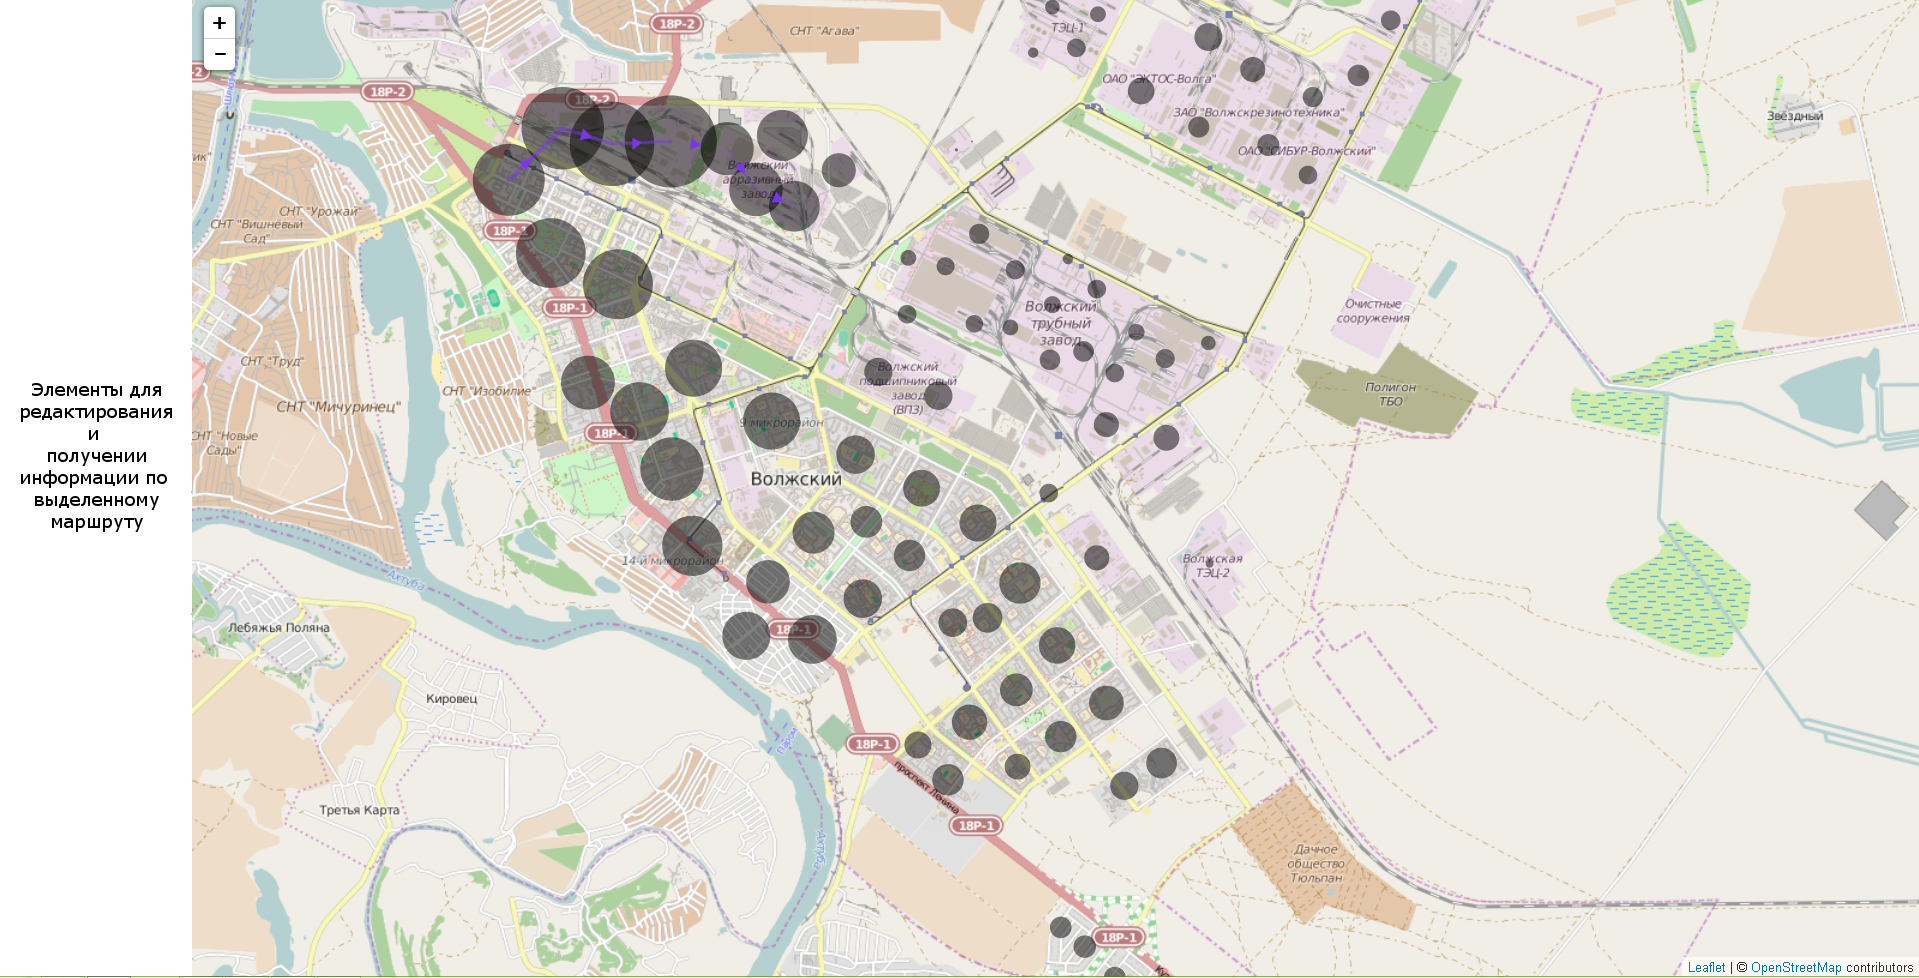
\includegraphics[width=\textwidth]{ui}
\end{figure}

\noindent
\emph{Реализованный алгоритм:} \url{https://github.com/vstu-cad-stuff/routing}\\
\emph{Текущая реализация:} \url{http://vstu-cad-stuff.github.io/routing/experimental/}\\

\newpage

\section{Псевдокод поглощающего алгоритма}\label{ref:greedy}
\noindent
1. \textbf{ВВОД} количество\_маршрутов, максимальная длина\\
2. \textbf{ДЕЛАТЬ ПОКА} маршрут < количество\_маршрутов:\\
3. \hspace*{0.5cm}\textbf{НАЙТИ} ребро графа с максимальной потребностью\\
4. \hspace*{0.5cm}\textbf{ВЫБРАТЬ} вершину с большим числом людей\\
5. \hspace*{0.5cm}\textbf{ДЕЛАТЬ ПОКА} длина != максимальная\_длина:\\
6. \hspace*{1.0cm}\textbf{ВЫБРАТЬ} ребро с максимальной потребностью\\
7. \hspace*{1.0cm}\textbf{ПЕРЕЙТИ} в вершину\\
8. \hspace*{1.0cm}длина += 1\\
9. \hspace*{0.5cm}маршрут += 1\\

\section{Псевдокод алгоритма имитации отжига}\label{ref:annealing}
\noindent
1. \( S \leftarrow \) начальное решение\\
2. \textbf{repeat}\\
3. \hspace*{2em} \textbf{выбрать} случайное решение \( R \) из окружение \( S \)\\
4. \hspace*{2em} \( \Delta \leftarrow f(R) - f(S) \)\\
5. \hspace*{2em} \textbf{if} \( \Delta < 0 \) \textbf{then} заменить \( S \) на \( R \)\\
6. \hspace*{2em} \textbf{else} заменить \( S \) на \( R \) c вероятностью \( e^{-\Delta/T} \)\\
7. \textbf{return} \( S \)

\newpage

\section{Псевдокод алгоритма поиска с запретами}\label{ref:tabu}
\noindent
1. \( l \leftarrow \) требуемая длина списка запретов\\
2. \( n \leftarrow \) количество модификаций\\
3. \( S \leftarrow \) начальное решение\\
4. \( B \leftarrow S \)\\
5. \( L \leftarrow { S } \) список запретов длины \( l \) с записанным \( S \)\\
6. \textbf{repeat}\\
7. \hspace*{2em} \textbf{if} Length(L) > l \textbf{then} удалить самый старый элемент из \( L \) \\
8. \hspace*{2em} \textbf{выбрать} решение \( R \) из \( S \)\\
9. \hspace*{2em} \textbf{for} n-1 \textbf{do}\\
10. \hspace*{4em} \textbf{выбрать} решение \( W \) из \( S \)\\
11. \hspace*{4em} \textbf{if} \( W \notin L \) и (\( f(W) > f(R) \) или \( R \in L \) ) \textbf{then} \( R \leftarrow W \)\\
12. \hspace*{4em} \textbf{if} \( R \notin L \) и \( f(R) > f(S) \) \textbf{then}\\
13. \hspace*{6em} \( S \leftarrow R \)\\
14. \hspace*{6em} \textbf{записать} \( R \) в \( L \)\\
15. \hspace*{4em} \textbf{endif}\\
16. \hspace*{2em} \textbf{if} \( f(S) > f(B) \) \textbf{then} \( B \leftarrow S \)\\
17. \textbf{until} достигнут предел по количеству итераций\\
18. \textbf{return} \( B \)\\